% \documentclass[handout]{beamer}
\documentclass{beamer}

\mode<presentation>
{
  \usetheme{default}
  \usefonttheme[onlymath]{serif}
  % \usetheme{Singapore}
  % \usetheme{Warsaw}
  % \usetheme{Malmoe}
  % \useinnertheme{circles}
  % \useoutertheme{infolines}
  % \useinnertheme{rounded}

  \setbeamercovered{transparent=5}
}

\usepackage[english]{babel}
\usepackage[latin1]{inputenc}
\usepackage{textpos,alltt,listings,multirow,ulem,siunitx}
\usepackage{pdfpages}
\newcommand\hmmax{0}
\newcommand\bmmax{0}
\usepackage{bm}

% font definitions, try \usepackage{ae} instead of the following
% three lines if you don't like this look
\usepackage{mathptmx}
\usepackage[scaled=.90]{helvet}
% \usepackage{courier}
\usepackage[T1]{fontenc}
\usepackage{tikz}
\usetikzlibrary[shapes,shapes.arrows,arrows,shapes.misc,fit,positioning]

% \usepackage{pgfpages}
% \pgfpagesuselayout{4 on 1}[a4paper,landscape,border shrink=5mm]

\usepackage{JedMacros}

\title{Toward less synchronous composable multilevel methods for implicit multiphysics simulation}
\author{Jed Brown\inst{1}, Mark Adams\inst{2}, Peter Brune\inst{1}, Matt Knepley\inst{3}, Dave May\inst{4}, Barry Smith\inst{1}}


% - Use the \inst command only if there are several affiliations.
% - Keep it simple, no one is interested in your street address.
\institute
{
  \inst{1}{Mathematics and Computer Science Division, Argonne National Laboratory} \\
  \inst{2}{Columbia University} \\
  \inst{3}{Computation Institute, University of Chicago} \\
  \inst{4}{ETH Z\"urich}
}

\date{2012-02-06}

% This is only inserted into the PDF information catalog. Can be left
% out.
\subject{Talks}


% If you have a file called "university-logo-filename.xxx", where xxx
% is a graphic format that can be processed by latex or pdflatex,
% resp., then you can add a logo as follows:

% \pgfdeclareimage[height=0.5cm]{university-logo}{university-logo-filename}
% \logo{\pgfuseimage{university-logo}}



% Delete this, if you do not want the table of contents to pop up at
% the beginning of each subsection:
% \AtBeginSubsection[]
% {
% \begin{frame}<beamer>
%   \frametitle{Outline}
%   \tableofcontents[currentsection,currentsubsection]
% \end{frame}
% }

\AtBeginSection[]
{
  \begin{frame}<beamer>
    \frametitle{Outline}
    \tableofcontents[currentsection]
  \end{frame}
}

% If you wish to uncover everything in a step-wise fashion, uncomment
% the following command:

% \beamerdefaultoverlayspecification{<+->}

\begin{document}
\lstset{language=C}
\normalem

\begin{frame}
  \titlepage
\end{frame}

\section{Multiphysics and methods}
\begin{frame}{Multiphysics problems}
  \begin{block}{Examples}
    \begin{itemize}
    \item Saddle-point problems (\eg incompressibility, contact)
    \item Stiff waves (\eg low-Mach combustion)
    \item Mixed type (\eg radiation hydrodynamics, ALE free-surface flows)
    \item Multi-domain problems (\eg fluid-structure interaction)
    \item Full space PDE-constrained optimization
    \end{itemize}
  \end{block}
  \begin{block}{Software/algorithmic considerations}
    \begin{itemize}
    \item Separate groups develop different ``physics'' components
    \item Do not know a priori which methods will have good algorithmic properties
    \item Achieving high throughput is more complicated
    \item Multiple time and/or spatial scales
      \begin{itemize}
      \item Splitting methods are delicate, often not in asymptotic regime
      \item Strongest nonlinearities usually non-stiff: prefer explicit for TVD limiters/shocks
      \end{itemize}
    \end{itemize}
  \end{block}
\end{frame}

\begin{frame}{The Great Solver Schism: Monolithic or Split?}
  \begin{columns}
    \begin{column}{0.5\textwidth}
      \begin{block}{Monolithic}
        \begin{itemize}
        \item Direct solvers
        \item Coupled Schwarz
        \item Coupled Neumann-Neumann \\
          (need unassembled matrices)
        \item Coupled multigrid
        \item[X] Need to understand local spectral and compatibility properties of the coupled system
        \end{itemize}
      \end{block}
    \end{column}
    \begin{column}{0.5\textwidth}
      \begin{block}{Split}
        \begin{itemize}
        \item Physics-split Schwarz \\
          (based on relaxation)
        \item Physics-split Schur \\
          (based on factorization)
          \begin{itemize}
          \item  approximate commutators \\
            SIMPLE, PCD, LSC
          \item segregated smoothers
          \item Augmented Lagrangian
          \item ``parabolization'' for stiff waves
          \end{itemize}
        \item[X] Need to understand global coupling strengths
        \end{itemize}
      \end{block}
    \end{column}
  \end{columns}
  \begin{itemize}
  \item Preferred data structures depend on which method is used.
  \item Interplay with geometric multigrid.
  \end{itemize}
\end{frame}

\begin{frame}{Splitting for Multiphysics}
  \begin{equation*}
    \begin{bmatrix}
      A & B \\ C & D
    \end{bmatrix}
    \begin{bmatrix}
      x \\ y
    \end{bmatrix}
    =
    \begin{bmatrix}
      f \\ g
    \end{bmatrix}
  \end{equation*}
  \begin{itemize}\item Relaxation:
    \code{-pc\_fieldsplit\_type [additive,multiplicative,symmetric\_multiplicative]}
    \begin{equation*}
      \begin{bmatrix}
        A & \\  & D
      \end{bmatrix}^{-1} \qquad 
      \begin{bmatrix}
        A & \\ C & D
      \end{bmatrix}^{-1} \qquad
      \begin{bmatrix}
        A & \\  & \bm 1
      \end{bmatrix}^{-1}
      \left(
        \bm 1 -
        \begin{bmatrix}
          A & B \\ & \bm 1
        \end{bmatrix}
        \begin{bmatrix}
          A & \\ C & D
        \end{bmatrix}^{-1}
      \right)
    \end{equation*}
    \begin{itemize}
    \item Gauss-Seidel inspired, works when fields are loosely coupled
    \end{itemize}
  \item Factorization: \code{-pc\_fieldsplit\_type schur}
    \begin{align*}
      \begin{bmatrix}
        A & B \\ & S
      \end{bmatrix}^{-1}
      \begin{bmatrix}
        1 & \\ CA^{-1} & 1
      \end{bmatrix}^{-1}, \qquad
      S = D - C A^{-1} B
    \end{align*}
    \begin{itemize}
    \item robust (exact factorization), can often drop lower block
    \item how to precondition $S$ which is usually dense?
      \begin{itemize}
      \item interpret as differential operators, use approximate commutators
      \end{itemize}
    \end{itemize}
  \end{itemize}
\end{frame}


\begin{frame}{How much nesting?}
  \begin{columns}
    \begin{column}{0.5\textwidth}
      \begin{equation*}
        P_1 =
        \begin{pmatrix}
          J_{uu} & J_{up} & J_{uE} \\
          0 & B_{pp} & 0 \\
          0 & 0 & J_{EE} \\
        \end{pmatrix}
      \end{equation*}
      \begin{itemize}
      \item $B_{pp}$ is a mass matrix in the pressure space weighted by inverse of kinematic viscosity.
      \item Elman, Mihajlovi\'c, Wathen, JCP 2011 for non-dimensional isoviscous Boussinesq.
      \item Works well for non-dimensional problems on the cube, not for realistic parameters.
      \end{itemize}
    \end{column}
    \begin{column}{0.5\textwidth}
      \begin{equation*}
        P =
        \begin{bmatrix}
          \begin{pmatrix}
            J_{uu} & J_{up} \\
            J_{pu} & 0
          \end{pmatrix} & \\
          \begin{pmatrix}
            J_{Eu} & J_{Ep}
          \end{pmatrix}
          & J_{EE}
        \end{bmatrix}
      \end{equation*}
      \begin{itemize}
      \item Inexact inner solve using upper-triangular with $B_{pp}$ for Schur.
      \item Another level of nesting.
      \item GCR tolerant of inexact inner solves.
      \item Outer converges in 1 or 2 iterations.
      \end{itemize}
    \end{column}
  \end{columns}
  \begin{itemize}
  \item Low-order preconditioning full-accuracy unassembled high order operator.
  \item Build these on command line with PETSc \cverb|PCFieldSplit|.
  \end{itemize}
\end{frame}

\begin{frame}[fragile]{Example $3\times 3$ problem with nested $2\times 2$ split}
\begin{Verbatim}[formatcom=\footnotesize]
-fieldsplit_s_ksp_type gcr
-fieldsplit_s_ksp_rtol 1e-1
-fieldsplit_s_ksp_monitor_vht
-fieldsplit_s_ksp_monitor_singular_value
-fieldsplit_s_pc_type fieldsplit
-fieldsplit_s_pc_fieldsplit_type schur
-fieldsplit_s_pc_fieldsplit_real_diagonal
-fieldsplit_s_pc_fieldsplit_schur_factorization_type lower
-fieldsplit_s_fieldsplit_u_ksp_type gmres
-fieldsplit_s_fieldsplit_u_ksp_max_it 10
-fieldsplit_s_fieldsplit_u_pc_type asm
-fieldsplit_s_fieldsplit_u_sub_pc_type ilu
-fieldsplit_s_fieldsplit_u_sub_pc_factor_levels 1
-fieldsplit_s_fieldsplit_u_ksp_converged_reason
-fieldsplit_s_fieldsplit_p_ksp_type preonly
-fieldsplit_s_fieldsplit_p_ksp_max_it 1
-fieldsplit_s_fieldsplit_p_pc_type jacobi
-fieldsplit_e_ksp_type gmres
-fieldsplit_e_ksp_converged_reason
-fieldsplit_e_pc_type asm
-fieldsplit_e_sub_pc_type ilu
-fieldsplit_e_sub_pc_factor_levels 2
\end{Verbatim}
\end{frame}

\begin{frame}[fragile]{Monolithic approaches}
  \begin{block}{Parallel direct solver}
    \begin{Verbatim}[formatcom=\footnotesize]
      -dm_mat_type aij -pc_type lu -pc_factor_mat_solver_package mumps
    \end{Verbatim}
  \end{block}
  \begin{block}{Coupled nonlinear multigrid accelerated by NGMRES with multi-stage smoothers}
  \begin{Verbatim}[formatcom=\footnotesize]
    -lidvelocity 200 -grashof 1e4
    -snes_grid_sequence 5 -snes_monitor -snes_view
    -snes_type ngmres
    -npc_snes_type fas
    -npc_snes_max_it 1
    -npc_fas_coarse_snes_type ls
    -npc_fas_coarse_ksp_type preonly
    -npc_fas_snes_type ms
    -npc_fas_snes_max_it 1
    -npc_fas_ksp_type preonly
    -npc_fas_pc_type pbjacobi
    -npc_fas_snes_ms_type m62
    -npc_fas_snes_max_it 1
  \end{Verbatim}
\end{block}
\end{frame}

\section{Coupling software in PETSc}
\begin{frame}{Multi-physics coupling in PETSc}
  \begin{columns}
    \begin{column}{0.5\textwidth}
      \tikzstyle{cloud} = [draw, ellipse,fill=red!20, node distance=3cm, minimum height=2em]
      \tikzstyle{block} = [rectangle, draw, fill=blue!20, text width=5em, text centered, rounded corners, minimum height=2em]
      \begin{tikzpicture}
        \node [cloud] (momentum) {Momentum};
        \node [cloud, right of=momentum] (pressure) {Pressure};
        \node<2-> [block, opacity=0.5, fit=(momentum)(pressure), text opacity=0.8] (stokes) {Stokes};
        \node<3-> [cloud, below=2em of momentum] (energy) {Energy};
        \node<3-> [cloud, below=2em of pressure] (geometry) {Geometry};
        \node<4-> [block, opacity=0.4, fit=(stokes)(momentum)(pressure)(energy)(geometry), text opacity=0.8, text height=4em] (ice) {Ice};
        \node<5-> [block, below=2em of ice, minimum width=16em] (bl) {{Boundary \nolinebreak Layer}};
        \node<5-> [block, below=2em of bl, minimum width=16em] (ocean) {Ocean};
        % ]
      \end{tikzpicture}
    \end{column}
    \begin{column}{0.5\textwidth}
      \begin{itemize}
      \item package each ``physics'' independently
      \item solve single-physics and coupled problems
      \item semi-implicit and fully implicit
      \item reuse residual and Jacobian evaluation unmodified
      \item direct solvers, fieldsplit inside multigrid, multigrid inside fieldsplit without recompilation
      \item use the best possible matrix format for each physics \\ (e.g. symmetric block size 3)
      \item matrix-free anywhere
      \item multiple levels of nesting
      \end{itemize}
    \end{column}
  \end{columns}
\end{frame}

\begin{frame}
  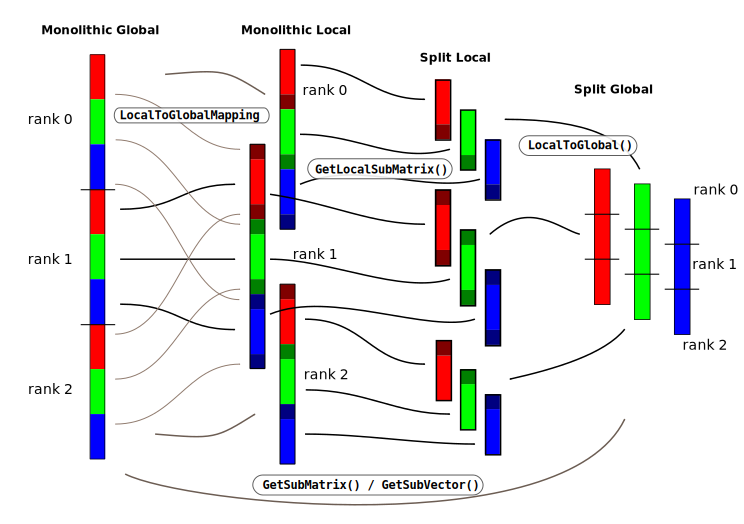
\includegraphics[width=\textwidth]{figures/PETSc/LocalSpaces} \\[-.5em]
  Work in Split Local space, matrix data structures reside in any space.
\end{frame}

\begin{frame}
  \alert{\texttt{MatGetLocalSubMatrix(Mat A,IS rows,IS cols,Mat *B);}}
  \begin{itemize}
  \item Primarily for assembly
    \begin{itemize}
    \item \texttt{B} is not guaranteed to implement \texttt{MatMult}
    \item The communicator for \texttt{B} is not specified, \\
      only safe to use non-collective ops (unless you check)
    \end{itemize}
  \item \texttt{IS} represents an index set, includes a block size and communicator
  \item \texttt{MatSetValuesBlockedLocal()} is implemented
  \item MatNest returns nested submatrix, no-copy
  \item No-copy for Neumann-Neumann formats \\ (unassembled across procs, e.g. BDDC, FETI-DP)
  \item Most other matrices return a lightweight proxy \texttt{Mat}
    \begin{itemize}
    \item \texttt{COMM\_SELF}
    \item Values not copied, does not implement \texttt{MatMult}
    \item Translates indices to the language of the parent matrix
    \item Multiple levels of nesting are flattened
    \end{itemize}
  \end{itemize}
\end{frame}

\setbeamertemplate{background canvas}{}
\includepdf[pages=1-3]{davemay.pdf}

\section{Hardware and consequences}
\begin{frame}{On-node hardware roadmap}
  \begin{block}{Hardware trends}
    \begin{itemize}
    \item More cores (keep hearing $\bigO(1000)$ per node)
    \item Long vector registers (32B for AVX and BG/Q, 64B for MIC)
    \item Must use SMT to hide memory latency (POWER7)
    \item Must use SMT for floating point performance (GPU, BG/Q)
    \item Large penalty for non-contiguous memory access
    \end{itemize}
  \end{block}
  \begin{block}{``Free flops'', but how can we use them?}
    \begin{itemize}
    \item High order methods good: better accuracy per storage
    \item High order methods bad: work unit gets larger
    \item GPU threads have very little memory, must keep work unit small
    \item Need library composability, keep user contribution embarrassingly parallel
    \end{itemize}
  \end{block}
\end{frame}

\begin{frame}{How to program this beast?}
  \begin{itemize}
  \item Decouple physics from discretization
    \begin{itemize*}
    \item Expose small, embarrassingly parallel operations to user
    \item Library schedules user threads for reuse between kernels
    \item User provides physics in kernels run at each quadrature point
    \item Continuous weak form: find $u \in \VV_D$
      \[ v^T F(u) \sim \int_\Omega v \cdot {\color{green!70!black} f_0(u,\nabla u)}
      + \nabla v \tcolon {\color{green!70!black} f_1(u,\nabla u)} = 0, \qquad \forall v \in \VV_0 \]
    \item Similar form at faces, may involve Riemann solve
    \end{itemize*}
  \item Library manages reductions
    \begin{itemize*}
    \item Interpolation and differentiation on elements
    \item Exploit tensor product structure to keep working set small
    \item Assembly into solution/residual vector (sum over elements)
    \end{itemize*}
  \end{itemize}
\end{frame}

\begin{frame}{Nodal $hp$-version finite element methods}
  \begin{columns}
    \begin{column}{0.4\textwidth}
      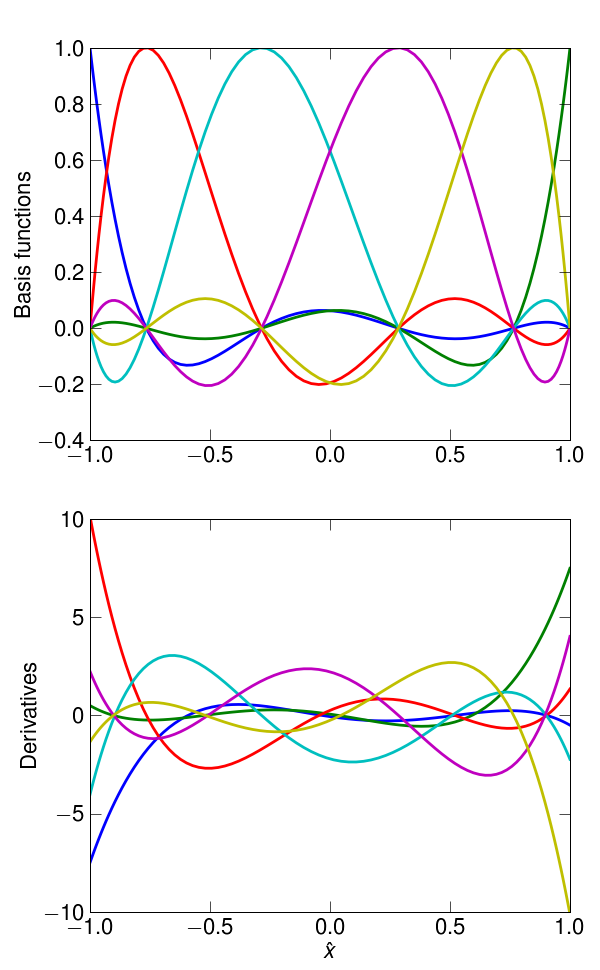
\includegraphics[width=\textwidth]{figures/lgl}
    \end{column}
    \begin{column}{0.6\textwidth}
      \begin{block}{1D reference element}
        \begin{itemize}
        \item Lagrange interpolants on Legendre-Gauss-Lobatto points
        \item Quadrature $\hat R$, weights $\hat W$
        \item Evaluation: $\hat B, \hat D$
        \end{itemize}
      \end{block}
      \vspace{-1em}
      \begin{block}{3D reference element}
      \vspace{-1em}
        \begin{align*}\label{eq:tprod}
          \begin{split}
            % \hat{\bm R} &= \hat R \otimes \hat R \otimes \hat R \\
            \hat{\bm W} &= \hat W \otimes \hat W \otimes \hat W \\
            \hat{\bm B} &= \alert<2>{\hat B \otimes \hat B \otimes \hat B} \\
          \end{split} &
          \begin{split}
            \hat{\bm D}_0 &= \alert<2>{\hat D \otimes \hat B \otimes \hat B} \\
            \hat{\bm D}_1 &= \alert<2>{\hat B \otimes \hat D \otimes \hat B} \\
            \hat{\bm D}_2 &= \alert<2>{\hat B \otimes \hat B \otimes \hat D} \\
          \end{split}
        \end{align*}
        \vspace{-1em}
        \begin{block}<2>{\alert{These tensor product operations \\ 
              are very efficient, 70\% of peak flop/s}}
        \end{block}
      \end{block}
    \end{column}
  \end{columns}
\end{frame}

\begin{frame}{Operations on physical elements}
  \begin{block}{Mapping to physical space}
    \vspace{-2em}
    \begin{gather*}
      x^e : \hat K \to K^e,\quad J^e_{ij} = \partial x_i^e/\partial \hat x_j, \quad (J^e)^{-1} = \partial \hat x/\partial x^e \\
    \end{gather*}
  \vspace{-2em}
  \end{block}
  \vspace{-2em}
  \begin{block}{Element operations in physical space}
  \vspace{-2em}
    \begin{align*}
      \bm B^e &= \hat{\bm B} \qquad \qquad \qquad \bm W^e = \hat{\bm W} \Lambda(\abs{J^e(\bm r)}) \\
      \bm D^e_i &= \Lambda\left(\frac{\partial \hat x_0}{\partial x_i}\right) \hat{\bm D}_0
      + \Lambda\left(\frac{\partial \hat x_1}{\partial x_i}\right) \hat{\bm D}_1
      + \Lambda\left(\frac{\partial \hat x_2}{\partial x_i}\right) \hat{\bm D}_2 \\
      (\bm D^e_i)^T &= \hat{\bm D}_0^T \Lambda\left(\frac{\partial \hat x_0}{\partial x_i}\right)
      + \hat{\bm D}_1^T \Lambda\left(\frac{\partial \hat x_1}{\partial x_i}\right)
      + \hat{\bm D}_2^T \Lambda\left(\frac{\partial \hat x_2}{\partial x_i}\right)
    \end{align*}
  \end{block}
  \vspace{-2em}
  \begin{block}{Global problem is defined by assembly}
  \vspace{-2em}
  \begin{equation*}
    F(u) =
    \sum_e \EE_e^T \Big[ (\bm B^e)^T \bm W^e \Lambda({\color{green!70!black} f_0(u^e,\nabla u^e)})
    + \sum_{i=0}^d(\bm D_i^e)^T \bm W^e \Lambda({\color{green!70!black} f_{1,i}(u^e,\nabla u^e)}) \Big] = \bm 0
  \end{equation*}
  where $u^e = \bm B^e \EE^e u$ and $\nabla u^e = \{\bm D_i^e \EE^e u\}_{i=0}^2$
  \end{block}
\end{frame}

\begin{frame}[shrink=5]{Representation of Jacobians, Automation}
  \begin{itemize}
  \item For unassembled representations, decomposition, and assembly
  \item Continuous weak form: find $u$
    \[ v^T F(u) \sim \int_\Omega v \cdot {\color{green!70!black} f_0(u,\nabla u)}
    + \nabla v \tcolon {\color{green!70!black} f_1(u,\nabla u)} = 0, \qquad \forall v \in \VV_0 \]
  \item Weak form of the Jacobian $J(u)$: find $w$
    \begin{gather*}
      v^T J(u) w \sim \int_\Omega \begin{bmatrix} v^T & \nabla v^T \end{bmatrix}
      {\color{blue} \begin{bmatrix} f_{0,0} & f_{0,1} \\ f_{1,0} & f_{1,1} \end{bmatrix}}
      \begin{bmatrix} w \\ \nabla w \end{bmatrix} \\
      {\color{blue} [f_{i,j}] = \begin{bmatrix} \dfrac{\partial f_0}{\partial u} & \dfrac{\partial f_0}{\partial \nabla u} \\[1em]
          \dfrac{\partial f_1}{\partial u} & \dfrac{\partial f_1}{\partial \nabla u} \end{bmatrix} (u,\nabla u) }
    \end{gather*}
  \item Terms in ${\color{blue} [f_{i,j}]}$ easy to compute symbolically, AD more scalable.
  \item Nonlinear terms ${\color{green!70!black}f_0,f_1}$ usually have the most expensive nonlinearities in the computation of scalars
    \begin{itemize}
    \item Equations of state, effective viscosity
    \item Compute gradient with reverse-mode, store at quadrature points.
    \item Perturb scalars, then use forward-mode to complete the Jacobian.
    \item Flip for action of the adjoint.
    \end{itemize}
  \end{itemize}
\end{frame}

\newcommand\smallterm[1]{{\color{gray} #1}}
\begin{frame}{Conservative (non-Boussinesq) two-phase ice flow}
  Find momentum density $\rho\uu$, pressure $p$, and total energy density $E$:
  \begin{gather*}
    (\rho\uu)_t + \div (\smallterm{\rho\uu\otimes\uu} - \eta D\uu_i + p\bm 1) - \rho \bm g = 0 \\
    \rho_t + \div \rho\uu = 0 \\
    E_t + \div \big((E+p)\uu - k_T\nabla T - k_\omega\nabla\omega \big) - \eta D\uu_i\tcolon D\uu_i - \smallterm{\rho\uu\cdot\bm g} = 0
  \end{gather*}
\begin{itemize}
\item Solve for density $\rho$, ice velocity $\uu_i$, temperature $T$, and melt fraction $\omega$ using constitutive relations.
  \begin{itemize}
  \item Simplified constitutive relations can be solved explicitly.
  \item Temperature, moisture, and strain-rate dependent rheology $\eta$.
  \item High order FEM, typically $Q_3$ momentum \& energy
  \end{itemize}
\item DAEs solved implicitly after semidiscretizing in space.
\item Preconditioning using nested fieldsplit
\end{itemize}
\end{frame}
\begin{frame}[shrink=5]{Performance of assembled versus unassembled}
  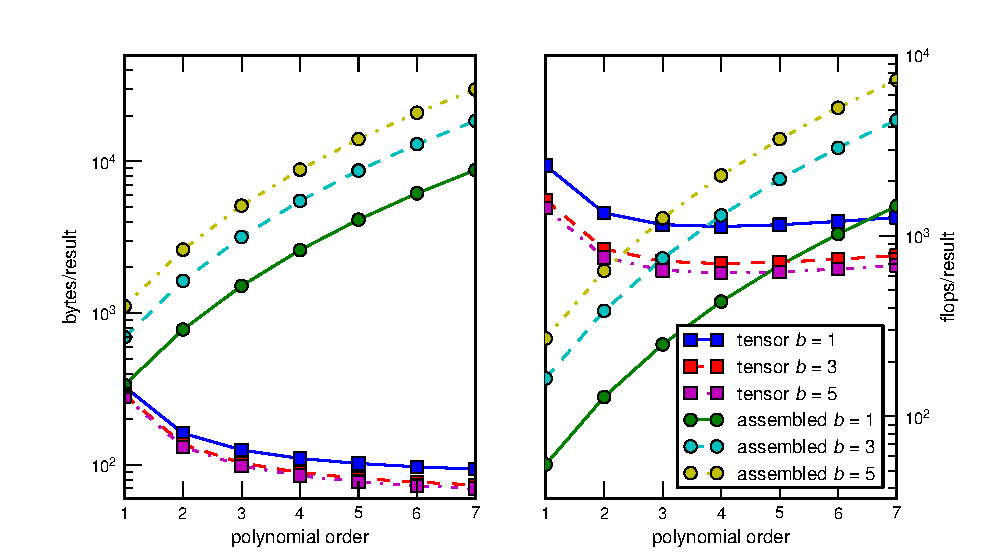
\includegraphics[width=\textwidth]{figures/TensorVsAssembly} \\
  \begin{itemize}
  \item High order Jacobian stored unassembled using coefficients at quadrature points, can use local AD
  \item Choose approximation order at run-time, independent for each field
  \item Precondition high order using assembled lowest order method
  \item Implementation $> 70\%$ of FPU peak, SpMV bandwidth wall $< 4\%$
  \end{itemize}
\end{frame}


\begin{frame}{Hardware Arithmetic Intensity}
  \begin{tabular}{lc}
    \toprule
    Operation                         & Arithmetic Intensity (flops per byte) \\
    \midrule
    Sparse matrix-vector product      & 1/6                  \\
    Dense matrix-vector product       & 1/4                  \\
    Unassembled matrix-vector product & $\approx 8$          \\
    High-order residual evaluation    & $> 5$                \\
    \bottomrule
  \end{tabular}
  \bigskip
  \begin{tabular}{lrrr}
    \toprule
    Processor           & BW (GB/s) & Peak (GF/s) & Balanced AI (F/B) \\
    \midrule
    Sandy Bridge 6-core & 21*       & 150         & 7.2                 \\
    Magny Cours 16-core & 42*       & 281         & 6.7                 \\
    Blue Gene/Q node    & 43        & 205         & 4.8                 \\
    GeForce 9400M       & 21        & 54          & 2.6                 \\
    GTX 285             & 159       & 1062        & 6.8                 \\
    Tesla M2050         & 144       & 1030        & 7.1                 \\
    \bottomrule
  \end{tabular}
\end{frame}


\begin{frame}{Prospects for reducing synchronization}
  \begin{itemize}
  \item Dot products and norms
    \begin{itemize}
    \item orthogonality is a powerful concept
    \item dot product/norm fusion in CG variants
    \item latency-tolerant Krylov methods, TSQR for GMRES
    \item nonlinear methods (e.g. NGMRES, BFGS, line searches)
    \item hierarchical methods to limit system-wide norms
    \item setting up smoothers and coarsening rates for AMG
    \end{itemize}
  \item additive coarse grids
  \item subphysics on subcommunicators, even within multigrid context
  \item $s$-step methods (and other fusion)
    \begin{itemize}
    \item often spoiled by algorithmic requirements of preconditioning
    \item relevant for multigrid smoothers
    \item difficult crossovers for 3D problems
    \end{itemize}
  \end{itemize}
\end{frame}

% \begin{frame}{$S$-step methods in 3D}
%   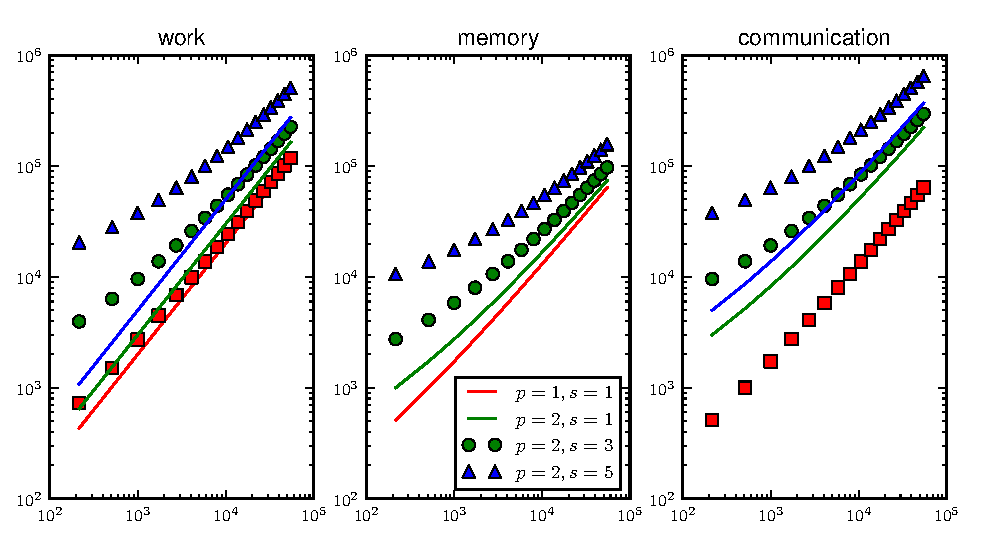
\includegraphics[width=1.1\textwidth]{figures/SStep.pdf}
% \end{frame}

\begin{frame}{Multigrid is \emph{always} strong scaling}
  \begin{itemize}
  \item Finest level is chosen by the application (might have big subdomains)
  \item All coarsened levels choose communicator size based on strong scaling limit
  \item Optimizing the strong scaling limit pays off consistently
  \item Rapid coarsening is important (2:1 semi-coarsening not okay any more)
  \end{itemize}
\end{frame}

\begin{frame}{Advanced Analysis}
  \begin{itemize}
  \item Uncertainty quantification
    \begin{itemize}
    \item intrusive vs unintrusive methods, multilevel
    \item uncertainty in modeling error
    \item use subdifferentials for non-smooth processes
    \item unified handling of heterogeneous observational data
    \end{itemize}
  \item PDE-constrained optimization
    \begin{itemize}
    \item multi-objective
    \item robustness
    \item rich problem description
    \item fusing algorithmic steps (LNK and coupled DD fuse gradients with progress)
    \end{itemize}
  \item Exploring stability manifolds
    \begin{itemize}
    \item solving bordered linear and nonlinear systems
    \end{itemize}
  \item nearly time-periodic nonlinear problems
    \begin{itemize}
    \item identifying cycles in ocean models, turbomachinery
    \end{itemize}
  \end{itemize}
\end{frame}

\begin{frame}{Software challenges}
  \begin{itemize}
  \item Which interfaces do users have to interact with?
    \begin{itemize}
    \item ``F''ramework vs library
    \item Extensibility is critical for multiphysics
    \end{itemize}
  \item Asynchronous interfaces crossing module boundaries
    \begin{itemize}
    \item How to ensure progress?
    \end{itemize}
  \item Merge communication on multiple levels or between multiple physics
  \item Fusing coarse level operations
  \item Working with non-nested communicators is tricky
  \item Current solutions for hierarchical memory are bad for libraries
    \begin{itemize}
    \item I want a communicator-like object
    \item I want a way to allocate memory explicitly/relative to algorithmic dependencies instead of implicit ``first touch''
    \end{itemize}
  \item Time integration: IMEX, multirate, parallel in time
    \begin{itemize}
    \item method of lines: $g(\dot u,u,t) = f(u,t)$
    \item Lax-Wendroff time integration is harder for composable software
    \end{itemize}
  \end{itemize}
\end{frame}

\end{document}
